\chapter{Mise en pratique}
Dans ce chapitre, j'utiliserai plusieurs appels système et implémenterai un petit programme en C afin d'observer de plus près le fonctionnement des pseudo-terminaux. Le but ici n'est en aucun cas de recréer quelque chose qui existe déjà. Autrement dit, je ne vais pas créer un pseudo-terminal et le manipuler, puisque je peux déjà utiliser les pseudo-terminaux directement créés par le noyau. Ainsi, les appels système tels que \texttt{posix\_openpty()}, \texttt{forkpty()}, etc., expliqués dans le livre de \textit{Michael Kerrisk}, ne seront pas utilisés. L'objectif concret est de 'fouiller' et voir comment tout fonctionne, tout en ayant un esprit critique à son égard.

\begin{tcolorbox}[title=Nota bene, colback=red!20]
Le programme implémenté ne fonctionnera pas sur le système d'exploitation Windows\texttrademark{}, car celui-ci n'utilise pas les pseudo-terminaux ou les utilise d'une autre manière. Concernant MacOS\texttrademark{}, celui-ci utilise bel et bien les pseudo-terminaux, mais d'une autre manière qui ressemble très fort au \textit{BSD-style} (voir chapitres précédents).
\end{tcolorbox}

\textcolor{red}{\textbf{Le programme a été testé et utilisé sur une distribution OpenSUSE (version 15.4) avec l'environnement de bureau KDE Plasma.}}

\vspace{\baselineskip}

Maintenant, le fonctionnement des pseudo-terminaux n'est plus un secret. Dans la très grosse majorité des distributions Linux, ce sont les pseudo-terminaux UNIX 98 qui sont utilisés, et c'est le noyau qui crée une nouvelle entrée dans le répertoire \textit{/dev/pts} lorsqu'il faut un pseudo-terminal. Ce programme va donc toujours utiliser les fichiers spéciaux qui se trouvent dans ce répertoire, d'où la petite mention \textit{Nota bene} au-dessus, entre autres.

\newpage

\section{Une lecture depuis le tampon d'entrée du pseudo-terminal esclave}
Est-ce que ce serait possible qu'on puisse lire depuis le tampon d'entrée d'un pseudo-terminal en cours d'utilisation sur le système ? On sait que le pseudo-terminal utilise deux tampons, un d'entrée et un autre de sortie. La réponse est \textbf{oui}.

Pour ce faire, il faut d'abord trouver où circulent les données, car on ne peut pas réellement accéder à ce tampon. Pour cela, un petit rappel concernant le terminal de contrôle. On avait vu que le terminal de contrôle gère les entrées, sorties et les \textit{jobs}. Le seul moyen de savoir quel est le terminal de contrôle du bash en cours d'utilisation, c'est d'utiliser la commande \textit{tty}. Une autre manière que je n'ai pas spécifiée, c'est aussi la commande \textit{ps aux} en regardant la colonne \textit{TTY}.

Une fois que le terminal de contrôle, qui est le pseudo-terminal esclave, est trouvé, il suffit d'effectuer une ouverture avec l'appel système \textit{open}, le but étant de récupérer le descripteur de fichier du pseudo-terminal esclave.

\begin{verbatim}
if( (fd = open(path, O_RDONLY)) < 0 ) {
                perror("open");
                exit(EXIT_FAILURE);
}
\end{verbatim}

Le \textit{path} est le chemin absolu vers le pseudo-terminal esclave (par exemple : /dev/pts/2). Ensuite, pour lire les entrées depuis le pseudo-terminal esclave, il faut utiliser l'appel système \textit{read}. Mais comme vu précédemment, le bash, qui est le \textit{programme lecteur}, ne lit les données de l'entrée uniquement si un caractère spécial qui joue le rôle de délimiteur est spécifié. C'est le caractère spécial \textbf{EOF} (ou \textbackslash n). Il faut à tout prix éviter un blocage inutile, puisque \textit{read()} va bloquer tant qu'il n'y a pas de données disponibles. Pour y remédier, on utilise l'appel système \textit{select}.

L'appel système \textit{select} permet d'effectuer une surveillance sur des descripteurs de fichiers et d'avertir lorsqu'un ou plusieurs descripteurs sont prêts pour la lecture ou l'écriture. Ces descripteurs de fichiers, \textit{select} les stocke dans des structures \textbf{fd\_set}.

Deux macros sont utilisées pour cela, \textit{FD\_ZERO}, qui permet de nettoyer la structure, et \textit{FD\_SET}, qui permet d'ajouter un descripteur de fichier dans une structure.

\newpage

\begin{verbatim}
FD_ZERO(&readfds);
FD_SET(fd, &readfds);

while( (select(fd + 1, &readfds, NULL, NULL, NULL)) 
				> 0 && strncmp("q", bytes, 1) != 0) {
	read(fd, bytes, 1);
        write(1, bytes, sizeof(bytes));
        FD_ZERO(&readfds);
        FD_SET(fd, &readfds);
}
\end{verbatim}

Après cela, l'appel système \textit{select()} retournera le nombre de descripteurs de fichiers qui ont changé de statut, que ce soit dans la structure des descripteurs de fichiers pour la lecture ou l'écriture. Pour information, \textit{select()} peut effectuer une surveillance sur des descripteurs de fichiers pour la lecture ou l'écriture, il y a donc 2 structures d'ensembles.

On peut distinguer que des données ne sont pas lues et ne s'affichent pas sur le pseudo-terminal cible, c'est tout à fait normal. Quand le programme va lire le tampon d'entrée du pseudo-terminal cible, il va vider le tampon et le pseudo-terminal cible n'affichera pas les données, mais certaines données peuvent être lues directement par le pseudo-terminal cible. Ce phénomène est dû au fait que quand le programme va lire l'entrée, lorsqu'une nouvelle donnée sera entrée au clavier, le pseudo-terminal cible aura le temps de la lire à son tour et le programme ne connaîtra pas son existence, vu que le pseudo-terminal cible a vidé le tampon et que le programme se trouve avec un tampon d'entrée vide.

\begin{figure}[h]
        \centering
	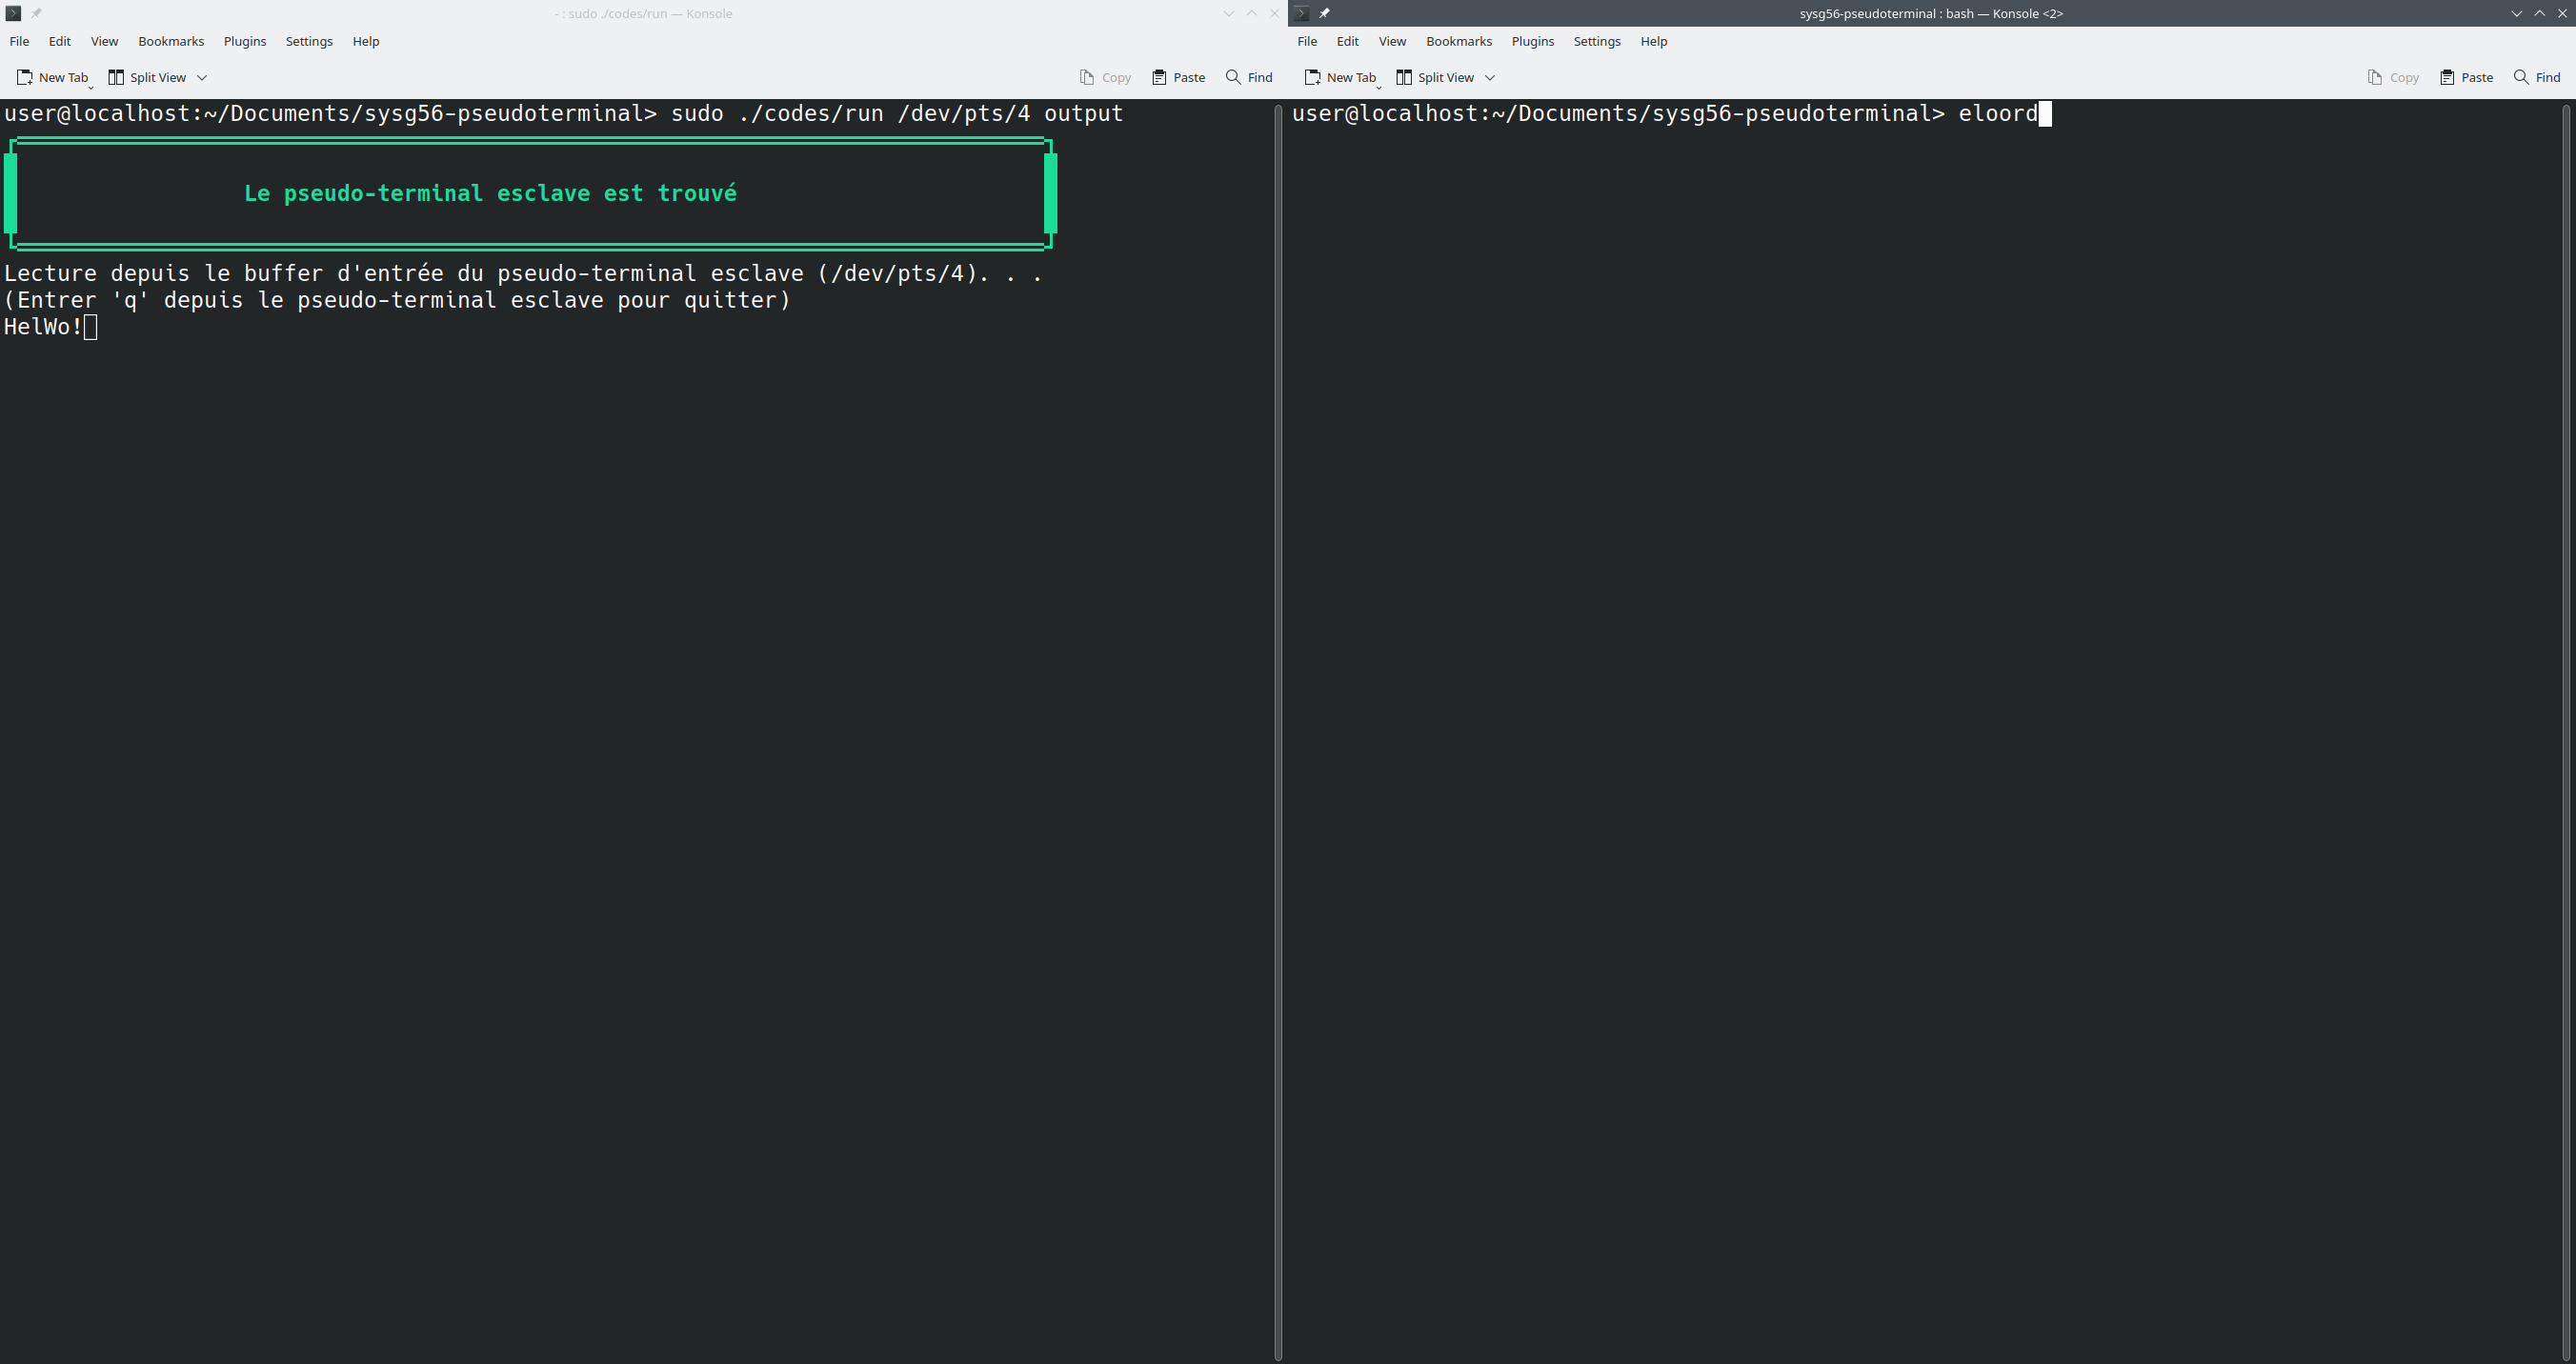
\includegraphics[width=250px, height=150px]{output.png}
	\caption{Exemple du programme (à gauche) qui lit l'entrée du pseudo-terminal esclave (à droite)}
\end{figure}

\section{Une écriture sur le tampon d'entrée du pseudo-terminal esclave}
Maintenant, on a vu que c'était possible de lire depuis le tampon d'entrée du pseudo-terminal esclave. Mais une autre étape à tester, c'est de voir si c'est possible d'écrire dans ce tampon. Sachant que le pseudo-terminal esclave fonctionne indépendamment de son côté en envoyant et recevant des données au maître, est-ce qu'un programme lambda peut directement altérer son fonctionnement et écrire dans ce tampon de telle sorte qu'une fois le pseudo-terminal esclave effectuera une lecture, il lira les données non pas reçues de la part du maître mais d'un programme extérieur.

Il est effectivement possible d'envoyer des données dans le tampon d'entrée du pseudo-terminal esclave. Il sera même possible de manipuler ce pseudo-terminal esclave comme si l'utilisateur interagissait directement avec lui. Bien sûr, que ce soit écrire ou lire (section précédente), il faut les droits root pour pouvoir utiliser le programme (et heureusement).

Pour ce faire, comme pour la section précédente pour la lecture, il faut d'abord ouvrir le pseudo-terminal esclave et récupérer son descripteur de fichier. Par la suite, il sera possible d'envoyer des données avec l'utilisation d'un appel système bien spécifique.

\begin{verbatim}
FD_ZERO(&writefds);
FD_SET(fd, &writefds);

while( (select(fd + 1, NULL, &writefds, NULL, NULL)) > 0 
                && ((messg = getchar()) != 'q') ) {
        if(ioctl(fd, TIOCSTI, &messg)) {
                        perror("ioctl");
                        exit(EXIT_FAILURE);
         }

FD_ZERO(&writefds);
FD_SET(fd, &writefds);
        }
\end{verbatim}

L'appel système en question est \textit{ioctl()}, qui permet de manipuler les paramètres d'un fichier spécial sous Linux. Petit rappel, dans les chapitres précédents, j'avais expliqué que le répertoire \textit{/dev} était un répertoire contenant des fichiers spéciaux. Et que ces fichiers étaient de types \textit{caractère} ou \textit{bloc}. Et l'appel système \textit{ioctl()} permet de manipuler ces fichiers spéciaux de type \textit{caractère}. Ça tombe bien, les pseudo-terminaux sont des fichiers spéciaux de types caractère.

\textit{man} est spécialement dédié aux pseudo-terminaux (\textit{man ioctl\_tty}). On peut y voir plusieurs commandes différentes qui permettent d'effectuer des opérations précises. La commande qui nous intéresse, c'est \textbf{TIOCSTI}.

\newpage

Une fois que les données seront stockées dans la variable \textit{messg} et que \textit{select()} avertira qu'une écriture est autorisée sur le pseudo-terminal esclave, l'appel système va envoyer les données stockées dans \textit{messg} dans le tampon d'entrée du pseudo-terminal esclave.

\begin{figure}[h]
        \centering
        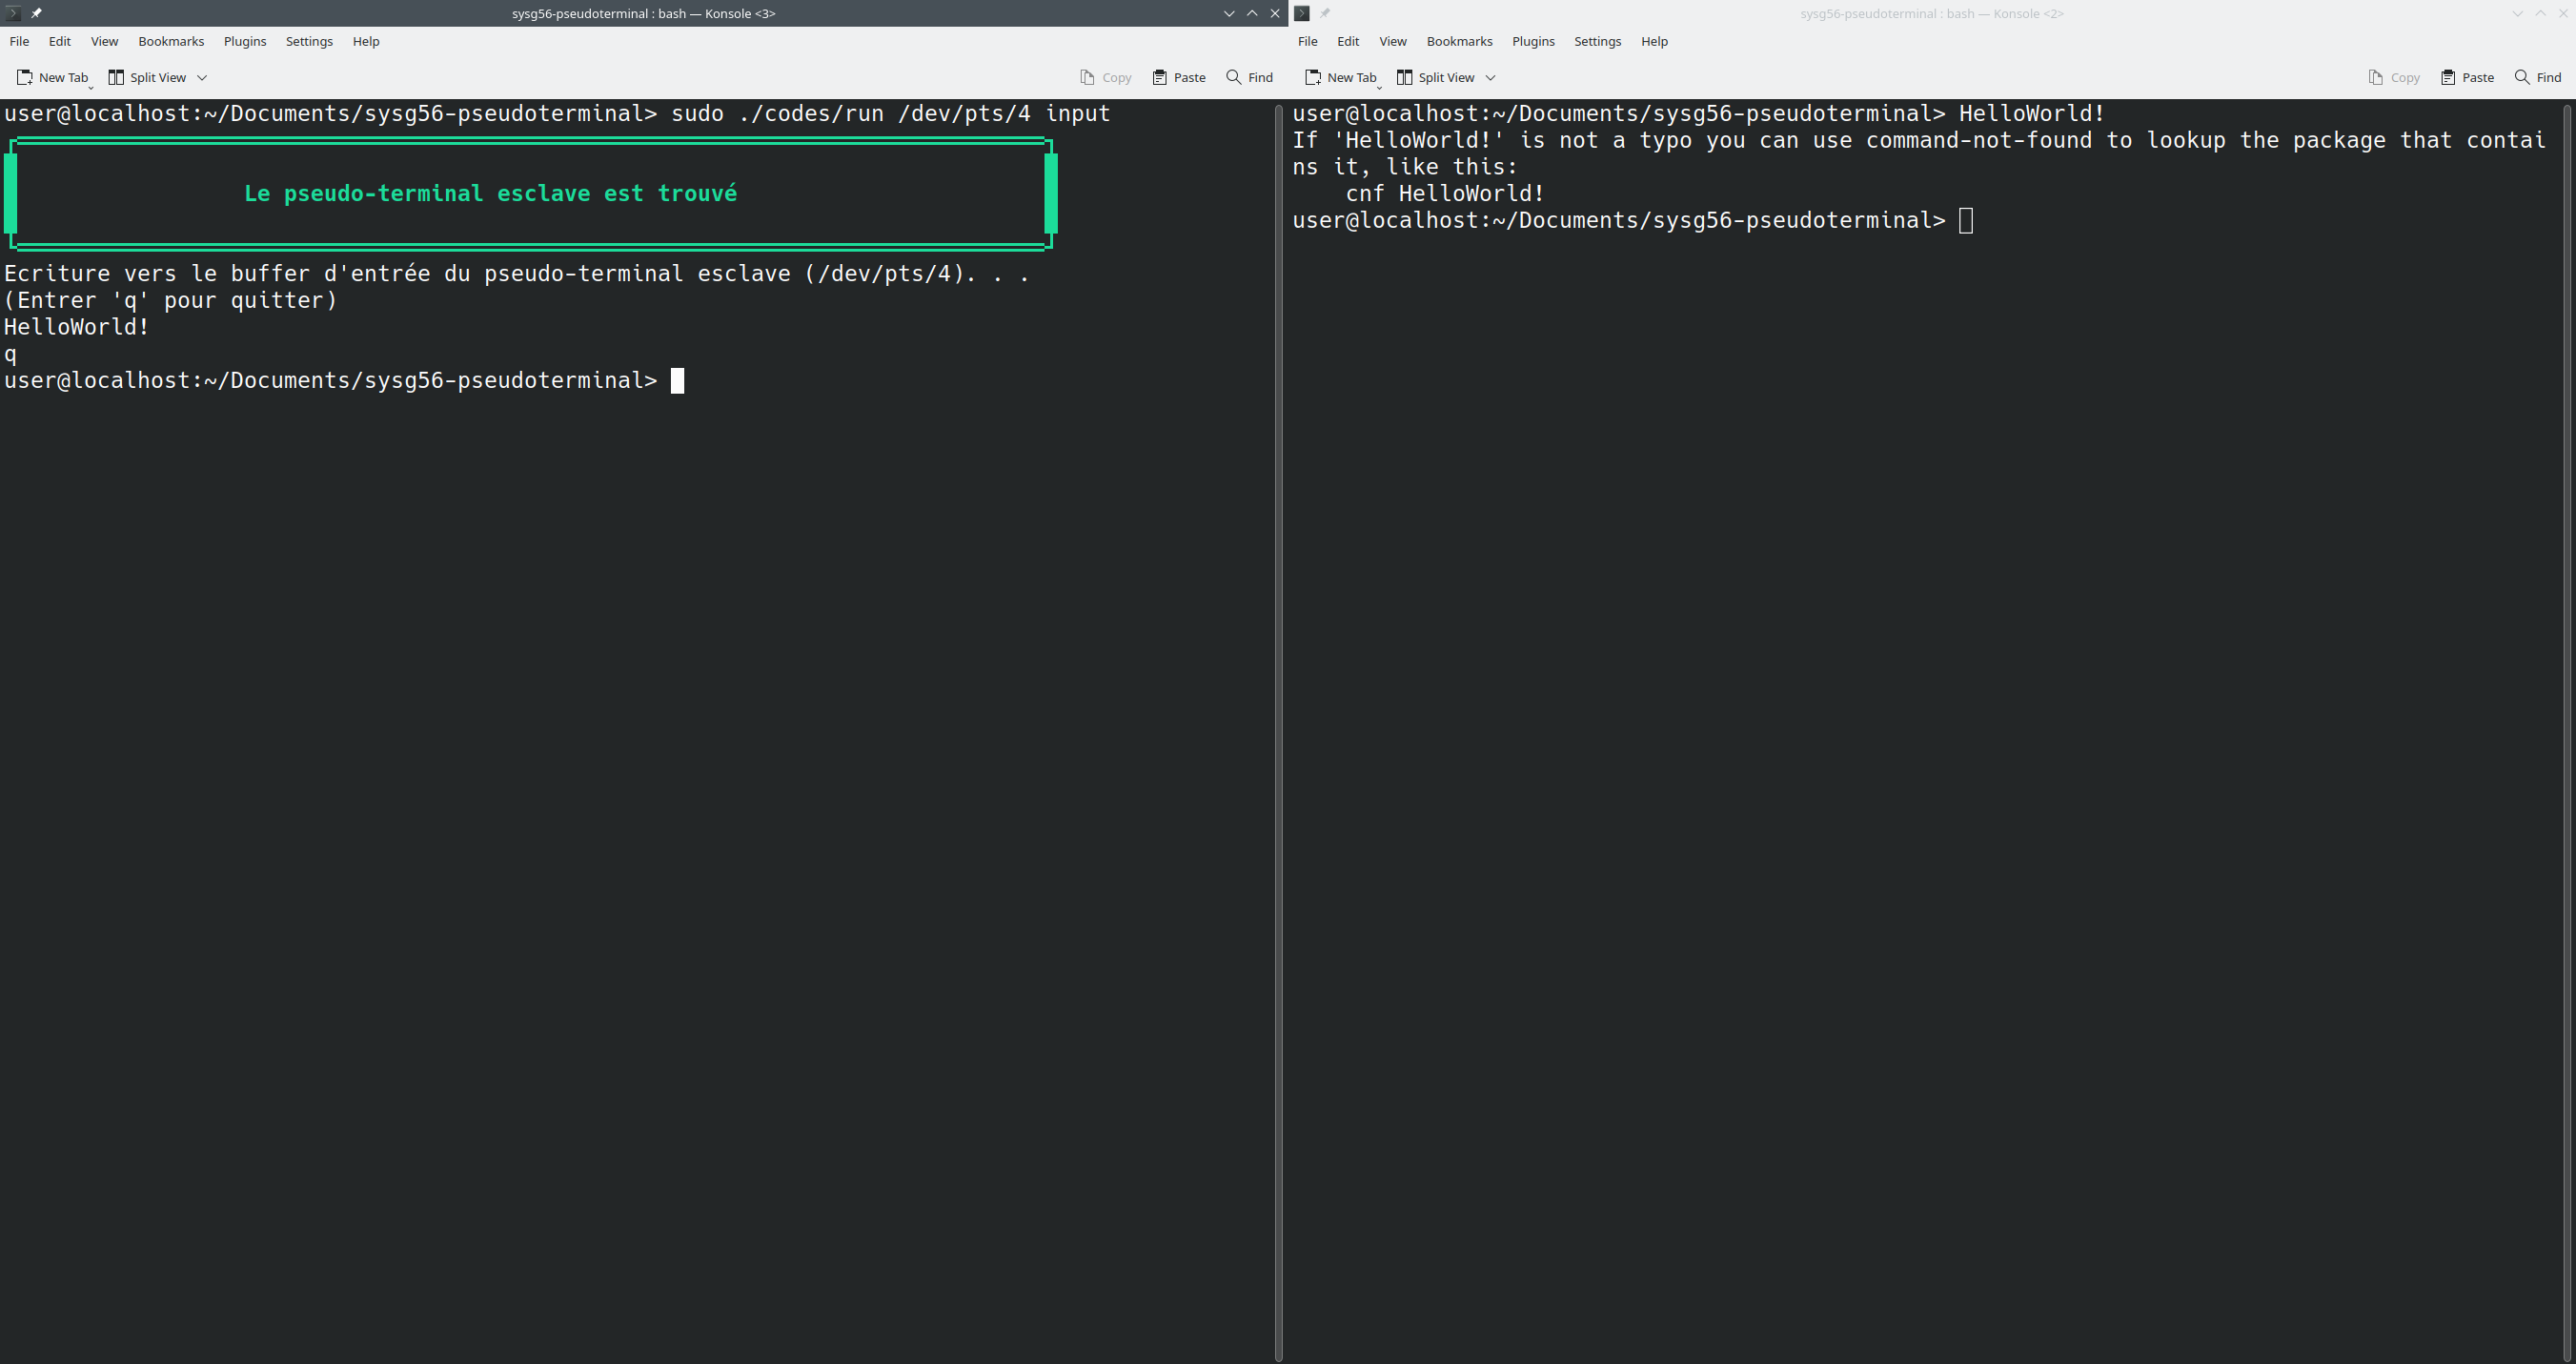
\includegraphics[width=250px, height=150px]{input.png}
        \caption{Exemple du programme (à gauche) qui écrit dans l'entrée du pseudo-terminal esclave (à droite)}
\end{figure}

\begin{tcolorbox}[title=Pour information]
	L'appel système \textit{ioctl} est très puissant. Il est aussi possible d'obtenir des informations à propos d'un pseudo-terminal, de récupérer la taille de la fenêtre du pseudo-terminal (en réalité, c'est la taille de la fenêtre de l'émulateur de terminal), de détacher le terminal de contrôle d'un processus et plein d'autres commandes très utiles...
\end{tcolorbox}

